\documentclass{article}
\usepackage[utf8]{inputenc}
\usepackage{array,multirow,graphicx}
\usepackage{amsmath,amssymb,latexsym}
\usepackage{mathabx}
\usepackage{parskip}
\usepackage{listings}
\usepackage[section]{placeins}
\usepackage{hyperref}
\usepackage[english]{babel}
\usepackage{biblatex}
\renewcommand{\sfdefault}{ptm}
\graphicspath{ {/} }

\title{Report.10.DB.Design.Magazine}
\author{Linh Duong}
\date{November 2017}

\begin{document}

\maketitle

\section{Database design}
\subsection{Determine concepts}
\begin{itemize}
    \item Magazine
    \item Article
    \item Author
\end{itemize}

\subsection{Determine attributes}
\begin{itemize}
    \item Magazine
    \subitem title
    \subitem ISSN
    \subitem order\_number
    \subitem year
    \subitem stored\_number
    
    \item Article
    \subitem title
    \subitem page of beginning
    \subitem page of ending 
    
    \item Author
    \subitem name
    \subitem e-mail address
    \subitem ascription

\end{itemize}

\section{Determine links}
\begin{itemize}
    \item Article and Magazine (has)
    \item Author and Article (has)
\end{itemize}

\section{Determine types}
\begin{itemize}
    \item Magazine
    \item Article
    \item Author
\end{itemize}

\section{Determine attributes}
\begin{itemize}
    \item Magazine
    \subitem title VARCHAR(200)
    \subitem ISSN VARCHAR(10)
    \subitem order\_number INT 
    \subitem stored\_number (INT)
    \subitem year (SMALLINT)
    
    \item Article
    \subitem title VARCHAR(200)
    \subitem page of beginning INT 
    \subitem page of ending INT
    
    \item Author
    \subitem name VARCHAR(50)
    \subitem e-mail address VARCHAR(50)
    \subitem ascription VARCHAR(50)
    
\end{itemize}

\section{Solve foreign key links}
\begin{itemize}
    \item Magazine
    \subitem maga\_id INT 
    \subitem order\_number INT 
    \subitem title VARCHAR(200)
    \subitem ISSN VARCHAR(10)
    \subitem stored\_number (INT)
    \subitem year (SMALLINT)
    
    \item Article
    \subitem article\_id INT
    \subitem maga\_id INT
    \subitem title VARCHAR(200)
    \subitem page of beginning INT 
    \subitem page of ending INT
    
    \item Author
    \subitem author\_id INT
    \subitem name VARCHAR(50)
    \subitem e-mail address VARCHAR(50)
    \subitem ascription VARCHAR(50)

    
    \item AuthorArticle
    \subitem author\_id INT
    \subitem article\_id INT
\end{itemize}

\section{Implementation}
\begin{lstlisting}[language=sql]
create database if not exists Magazines;

use magazines;

create table magazine (
maga_id int not null auto_increment, 
order_number int,
title varchar(200),
issn varchar(10),
stored_number int, 
year smallint,
primary key (maga_id)
);

create table article (
article_id int not null auto_increment, 
maga_id int ,
title varchar(200),
begin_page int, 
end_page int, 
primary key (article_id), 
foreign key (maga_id) references magazine(maga_id)
);

create table author (
author_id int not null auto_increment, 
name varchar(50), 
email varchar(50),
ascription varchar(50), 
primary key (author_id)
);

create table author_article (
author_id int, 
article_id int, 
foreign key (author_id) references author(author_id), 
foreign key (article_id) references article(article_id)
);
\end{lstlisting}

\section{Describe tables}
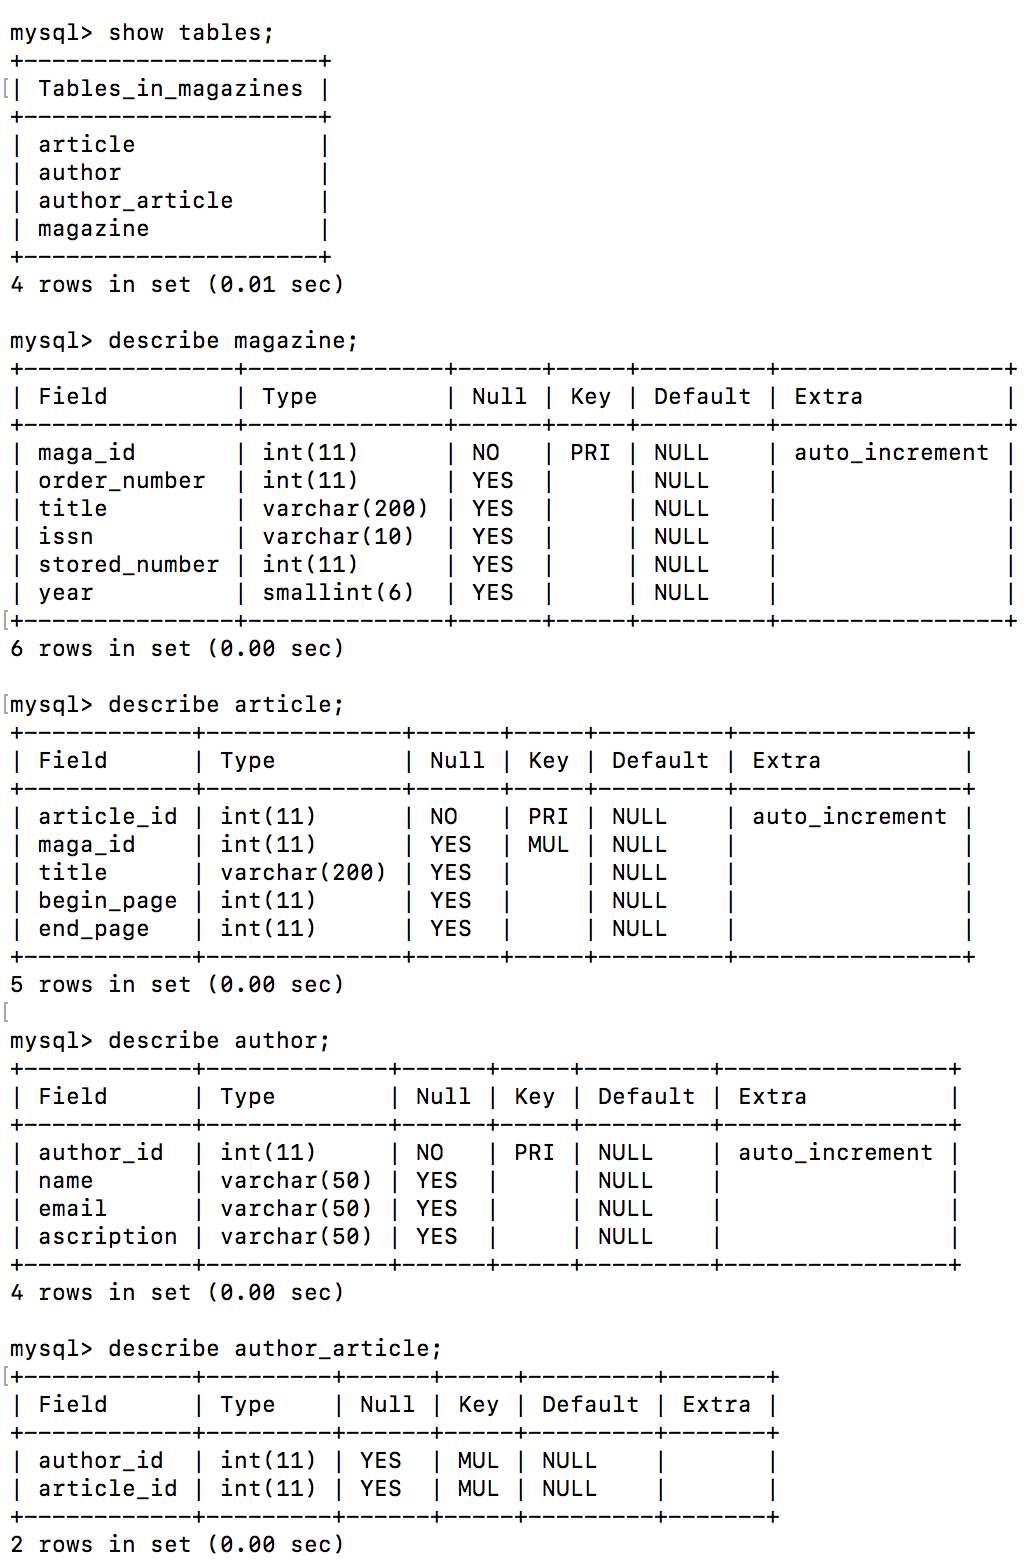
\includegraphics[width=\linewidth]{describe.png}



\end{document}
